\section{Selección de las muestras}\label{sec:2_muestras}

En esta sección se explica qué es el proyecto \hatlas\ y qué es el proyecto \gama, de qué instrumentos se sirven estos proyectos para realizar las medidas y que datos nos proporcionan. Por último, se mostrará la zona en la que se produce un solapamiento de ambos cartografiados que es la zona en la podemos aplicar nuestra propuesta para la identificación del SLGs.

\subsection{Proyecto \hatlas}

\hatlas\ (\anglicismo{Herschel} Astrophysical Terahertz Large Area Survey) es el nombre de uno de los proyectos astronómicos que se fundamenta en las medidas del telescopio espacial \h. Este proyecto cubre un área total de \maths{550\;\mathrm{deg}^{2}} (la octogésima parte del cielo) requiriendo unas 600 horas de observación, lo que implica un tiempo cuatro veces mayor que todas las demás prospecciones extragalácticas de \h\ combinadas. 
Con ello se espera detectar unas \maths{2,5\times10^{5}} galaxias con desplazamientos al rojo de hasta \maths{z\sim4}, cuando el Universo tenía apenas unos pocos miles de millones de años \citep{website:hatlas}.

\subsubsection{Observatorio espacial \h.}

El observatorio espacial \h\footnote{El satélite fue nombrado en honor al astrónomo británico William Herchel conocido entre otras cosas, por el descubrimiento del planeta Urano y del espectro infrarrojo. No confundir con el telescopio óptico e IR-cercano llamado William Herschel Telescope (W\textit{H}T) que se encuentra en el Observatorio del Roque de los Muchachos en la isla de La Palma.} es un proyecto de la ESA (European Space Agency), lanzado el día 14 de mayo de 2009 junto con el satélite espacial Planck. El periodo de vida útil terminó el día 29 de Abril de 2013 cuando agotaron los 2200 litros de helio superfluido que utilizaba como refrigerante. Se encontraba situado en el punto \maths{{L}_{2}} de Lagrange, a unos \maths{1.5 \times {10}^{6}\;\mathrm{km}} de la Tierra; este es un punto de especial interés para colocar observatorios espaciales, puesto que los cuerpos situados ahí mantienen la misma posición relativa entre el Sol y la Tierra.
Se trata del mayor telescopio infrarrojo espacial que se ha construido hasta el momento. Dispone de un único espejo de 3.5 metros de diámetro y de varios instrumentos diseñados para realizar observaciones en el rango espectral que va desde el IR lejano hasta la banda submilimétrica, \microm{55-672}. 

Los tres instrumentos del observatorio espacial son:

\vspace{-3mm}
\begin{itemize}
    
    \item \spire\ (Spectral and Photometric Imaging Receiver) \cite{website:spire_website}.
    
    Se trata de una cámara fotométrica y un espectrómetro de transformada de Fourier. Ambos instrumentos operaban refrigerados por He líquido superfluído a una temperatura de \maths{\sim~0.3\;\mathrm{K}}. \spire\ se construyó con dos objetivos, el estudio de la formación de estrellas y la formación de galaxias. En ambos casos está involucrado un proceso similar de absorción de la luz visible y UV procedente de las estrellas y posterior remisión de radiación IR por el gas y polvo interestelar, con una longitud de onda de unos \microm{100}.
    
    La cámara opera simultáneamente en tres bandas del espectro electromagnético, centradas en \microm{250}, \microm{350}, y \microm{500}, con una resolución angular de \maths{20-30\:\mathrm{arcsec}} y un campo de visión de \maths{4\times8} minutos de arco. El sensor cuenta con 270 píxeles.
    
    El espectrómetro tiene una resolución espectral de \maths{300\;\mathrm{km\;{s}^{-1}}}, cubre el rango de frecuencias entre \microm{200-670}   y su resolución angular es de \maths{20-50\:\mathrm{arcsec}}. El campo de visión es de \maths{2.6\times2.6} minutos de arco. En cuanto al detector, dispone de 56 píxeles.
     
    El instrumento ha sido construido por un consorcio internacional de 18 instituciones, de 8 países, liderado por el Dr. Matt Griffin del Cardiff Institute (AIG)\citep{website:h_instrumets}.
    
    \item \pacs\ (Photodetecting Array Camera and Spectrometer) \citep{website:pacs_website}.
    
    Al igual que \spire, \pacs\ está formado por dos instrumentos independientes; una cámara y un espectrómetro integral de campo. 
    
    La cámara toma imágenes en dos bandas de forma simultánea, a \microm{60-85} o \microm{85-130} y a \microm{130-210} mediante dos sensores bolométricos. Los sensores bolométricos están formados por un array de \maths{32\times16} y de \maths{64\times32} respectivamente. La resolución angular es de \maths{5\:\mathrm{arcsec}} y el campo de visión es de \maths{1.75\times3.5} minutos de arco. El límite de detección está en \maths{3\;m\mathrm{Jy}}\footnote{El Jansky (Jy) es una unidad de densidad de flujo espectral o irradiancia, especialmente utilizada en astronomía que no pertenece al Sistema Internacional de Unidades (SI). Es equivalente a \maths{{10}^{-26}\:\mathrm{W\:m^{-2} {Hz}^{-1}}}.}.
    
    Al espectrómetro también trabaja simultáneamente en dos frecuencias, en \microm{57-105} y \microm{105-210}. Los detectores están compuestos por un array de \maths{5\times5} y de \maths{16\times25} sensores de Ge-Ga. La resolución espectral es de \maths{150-200\;k\mathrm{m\;{s}^{-1}}}, la resolución espacial es de \maths{10\:\mathrm{arcsec}} y el campo de visión de \maths{50\times50}. Para \maths{\frac{\lambda}{\Delta \lambda}\sim1500} la sensibilidad es de \maths{5\times{10}^{-18}\mathrm{W\;{m}^{-2}}}.
    
    El instrumento ha sido construido por un consorcio internacional de 12 instituciones pertenecientes a 6 países, liderado por el investigador Dr. Albrecht Poglitsch del Max-Planck-Institute\citep{website:h_instrumets}.
    
    
    \item \hifi\ (Heterodyne Instrument for the Far Infrared) \citep{website:hifi_website}.
    
    Se trata de un espectrómetro de muy alta resolución espectral (0.02-0.7 km/s) que trabaja entre los \microm{157-625}. Tiene una resolución espacial de \maths{13-40\:\mathrm{arcsec}}. La temperatura de trabajo se encuentra entre los \kelvin{2-10}.
    
    Al igual que los instrumentos anteriores, este ha sido construido por un consorcio internacional de 26 instituciones pertenecientes a 11 países diferentes. El líder principal del proyecto en este caso es Thijs de Graauw del Stichting Ruimte Onderzoek Nederland (SRON)\citep{website:h_instrumets}.


\end{itemize}

\subsubsection{Catálogo \hatlas\ DR1.}\label{subsec:catalogo_hatlas}

El lanzamiento de datos \hatlas\ DR1 (Data Release 1) fue publicado el 28 de junio de 2016. Los detalles sobre su contenido se encuentran en las publicaciones \cite{article:valiente_2016} y
\cite{article:bourne_2016}. Este lanzamiento de datos incluye varios mapas y archivos adicionales; en este trabajo se utilizará únicamente el fichero {\small HATLAS\_DR1\_CATALOGUE\_V1.2.FITS}\footnote{Dirección de descarga: \url{http://www.h-atlas.org/public_data/DR1/HATLAS_DR1_CATALOGUE_V1.2.FITS}}.
Se compone de tres campos centrados en ascensión recta 09h, 12h y 14.5h sobre el ecuador celeste (denominadas por el proyecto Bloques, Figura~\ref{fig:TOPCAT_HATLAS}) que cubren cubren un área de total de  \maths{161\;\mathrm{{deg}^{2}}} con 120230 fuentes identificadas en 3 bandas fotométricas.

\begin{figure}[htb]
    \begin{center}
         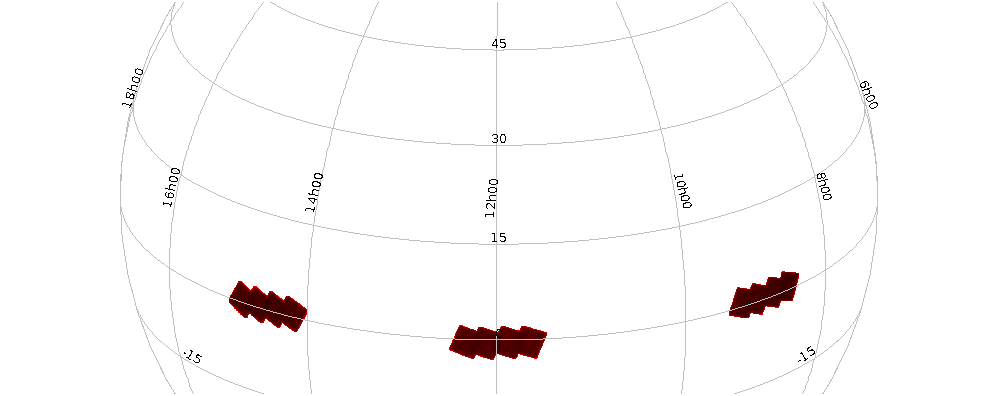
\includegraphics[width=14cm]{2_Muestras/atlas.png}
    \end{center}
    
    \caption{\small Representación de los objetos publicados en el catálogo \hatlas\ Data Release 1 (DR1) en coordenadas ecuatoriales utilizando el programa TOPCAT\footnotemark (Tool for OPerations on Catalogues And Tables). De derecha a izquierda, cada una de las tres regiones recibe el nombre de Bloque 2, Bloque 3 y Bloque 4. (ver: \href{website:hatlas_fields}{http://www.h-atlas.org/survey/fields})}.
    \label{fig:TOPCAT_HATLAS}
\end{figure}
\footnotetext{Página web del proyecto que desarrolla TOPCAT: \url{http://www.star.bris.ac.uk/\%7Embt/topcat/}}

A continuación se muestra una breve descripción de las columnas del catálogo\footnote{Para una descripción completa de cada una de las columnas del fichero consultar la dirección:

\url{http://www.h-atlas.org/public_data/DR1/HATLAS_DR1_CATALOGUE.COLUMNS}} que son relevantes en este trabajo:

\vspace{-3mm}
\begin{itemize}
    \setlength\itemsep{-1mm}
    \item HATLAS\_IAU\_ID: Contiene el identificador de la fuente astronómica del catálogo \hatlas\ asignado por la IAU (International Astronomy Union).
    \item RA: Ascensión recta, en grados, de la fuente astronómica obtenida a partir de los datos de la banda de \microm{250}.
    \item DEC: Declinación, en grados, de la fuente astronómica obtenida a partir de los datos de la banda de \microm{250}. 
    
    \item F250: Flujo de la fuente, en Jy, de la banda de \microm{250}.  El límite de detección \maths{5\sigma}\footnote{Una desviación estándar de \maths{1\sigma} significa que si asumimos una distribución normal de los valores posibles que puede tomar una medida respecto a su valor verdadero \maths{x}, hay un probabilidad de en torno al \maths{68\%} de que esta se encuentre en el intervalo \maths{x\pm\sigma}. El límite de detección \maths{5\sigma} es un criterio para determinar cuándo se ha detectado una fuente sobre la señal de ruido de fondo.} de esta banda se encuentra en \maths{33.5\;\mathrm{mJy}} \citep{article:Nuevo_2012}
    
    \item F350: Flujo, en Jy, de la banda de \microm{350}. El límite de detección \maths{5\sigma}, \maths{37.7\;\mathrm{mJy}}.
    
    \item F500: Flujo, en Jy, de la banda de \microm{500}. El límite de detección \maths{5\sigma}, \maths{44.0\;\mathrm{mJy}}.
    
    \item E250: Desviación estándar (\maths{1\sigma}) del flujo para la observación de un objeto en la banda \microm{250}. 
    \item E350: Desviación estándar del flujo en la banda \microm{350}.
    \item E500: Desviación estándar del flujo en la banda \microm{500}.
    \item \maths{\mathrm{GSQ\_FLAG}}: Se hace una clasificación del tipo de objeto basada diagramas de color g-i~/~J-K además de los criterios de PSF~/~magnitud de modelo de banda r \citep{article:bourne_2016}. La columna contiene un entero con tres posibles valores, cuyo significado es el  siguiente: 0=galaxia, 1=estrella, 2 y 3=cuásar.
    
    \item \maths{\mathrm{Z\_SPEC}}: Contiene los valores del \rt\ de algunos de los objetos del catálogo \hatlas. Aquellos cuyo valor es desconocido y no ha podido calcularse fotométricamente aparecen con valor -99.		
    \item \maths{\mathrm{Z\_QUAL}}: Etiqueta que indica el nivel de confianza \maths{Q_h} que se tiene sobre el valor del \rt\ que aparece en la columna \maths{\mathrm{Z\_SPEC}}. Los objetos cuya etiqueta tiene un valor \maths{\geq3}, tienen \anglicismo{redshifts} espectroscópicos considerados de confianza. El proyecto indica que los \anglicismo{redshifts} fotométricos han sido calculados mediante ANNz; por ese motivo hemos tratado a aquellas medidas con un factor de calidad 1 o 2 como si hubieran sido obtenidos mediante ANNz. 
    \item \maths{\mathrm{Z\_SOURCE}}: Indica la fuente de procedencia de los valores del \rt\ del catálogo. El código es el siguiente: 1- SDSS DR7, 2- 6dFGS, 4- 2SLAQ-QSO, 8- 2SLAQ-LRG, 16- GAMA HATLAS filler targets, 32- GAMA Main Survey, 64- 2dFGRS, 128- SDSS DR10, 256- Wigglez, 512- GAMA (que no se encuentran actualmente en TilingCat de GAMA-II)
\end{itemize}

\newpage

De las 120230 fuentes del catalogo DR1 solo 28389 tienen un \rt\ con factor de calidad \maths{Q_h\geq3} y 931 factor de calidad \maths{Q_h=1\vee2} (ver fig: \ref{fig:histograma_z_hatlas}). Al resto de fuentes, cuyo \rt\ es desconocido, les aplicaremos el algoritmo descrito en la sección \ref{sec:3_redshift_hatlas}. Si estos resultan ser galaxias (según la clasificación de la columna \maths{\mathrm{GSQ\_FLAG}}) y el ajuste proporciona un valor comprendido entre \maths{1<z<3.5} aceptaremos el valor del ajuste como medida válida de \maths{z}. 

En cuanto a la desviación estándar de las medidas del \rt\ el proyecto no proporciona su valor directamente. Para conocer su valor tendríamos que conocer los detalles de cómo se ha obtenido el \rt\ dependiendo de la procedencia de las medidas, lo cual implica mucho tiempo, que no está justificado emplear en este trabajo de final de grado. Una alternativa hubiera sido buscar los objetos en otra base de datos como NED (NASA/IPAC Extragalactic Database: \url{http://ned.ipac.caltech.edu/}) o SIMBAD (Set of Identifications, Measurements, and Bibliography for Astronomical Data: \url{http://simbad.u-strasbg.fr/simbad/}) ya que existen rutinas ya implementadas en \python\ para este tipo de tareas. Sin embargo, nos podemos encontrar en la situación de que estas bases de datos tampoco dispongan de las desviaciones estándar de todos los objetos en los que estamos interesados\footnote{Se ha realizado una búsqueda individual de unos cuantos objetos del catálogo \hatlas\ (30 objetos), cuyo \rt\ tiene \maths{Q_h\geq3} a partir del identificador asignado por la IAU en la base de datos NED y se ha encontrado el valor de \maths{z} y \maths{{\sigma}^{z}} solamente para unos pocos casos (3).}. Por ese motivo, la solución que se ha adoptado en este trabajo ha sido dividir las medidas proporcionadas por \hatlas\ en dos grupos. Por una parte tenemos los objetos cuyo factor de calidad es \maths{Q_h=1\vee2}. Estos objetos suponemos que se han obtenido todos ellos mediante ANNZ, por lo que si las medidas se encuentran en el rango \maths{0<z<0.7}, es razonable suponer para todas ellas  \maths{{\sigma}^{z}=0.023} a partir del estudio realizado por \cite{article:annz}. En el caso de que el factor de calidad sea \maths{Q_h\geq3} la desviación estándar de las medidas se obtendrá a partir del ajuste que se muestra en la Figura~\ref{fig:ajuste_error_gama} (asignar la misma desviación estándar a los desplazamientos al rojo espectroscópicos de los proyectos \gama\ y \hatlas\ está justificado porque la procedencia de estas medidas es la misma en muchos casos). El hecho de que una medida tenga un factor de calidad más alto que otra, no quiere decir que el valor de las desviaciones estándar sea diferente. El factor de calidad indica la confianza subjetiva que tienen los autores del catálogo sobre las medidas del \rt\ \citep{article:Driver_2011}. La confianza puede ser baja por cualquier motivo.

En resumen, para asignar los errores a las medidas del \rt\ de los objetos de \hatlas\, se ha decidido lo siguiente:

\vspace{-3mm}

\begin{itemize}
    \item Si el factor de calidad de la medida del \rt\ por el proyecto \hatlas\ es \maths{\geq3}, el \rt\ es espectroscópico y la desviación estándar se obtiene a partir de la expresión \maths{{\sigma}^{z}=1.1\times{10}^{-4}\times(1+z)}.
    
    \item Si el factor de calidad \maths{Q_h=1\vee2}, se tratará a la medida como si hubiera sido obtenida mediante ANNZ. Si su valor pertenece al intervalo \maths{0<z<0.7} se le asignará una desviación estándar \maths{{\sigma}^{z}=0.023}.
    
    \item Si el \rt\ es desconocido por el proyecto \hatlas\ y el ajuste obtenido mediante el algoritmo descrito en la Sección~\ref{sec:3_redshift_hatlas} se encuentra en el intervalo \maths{1<z<3.5} consideraremos válido este valor y le asignaremos una desviación estándar  \maths{{\sigma}^{z}=0.115\times(1+z)} .
\end{itemize}

\begin{figure}[htb]
    \begin{center}
         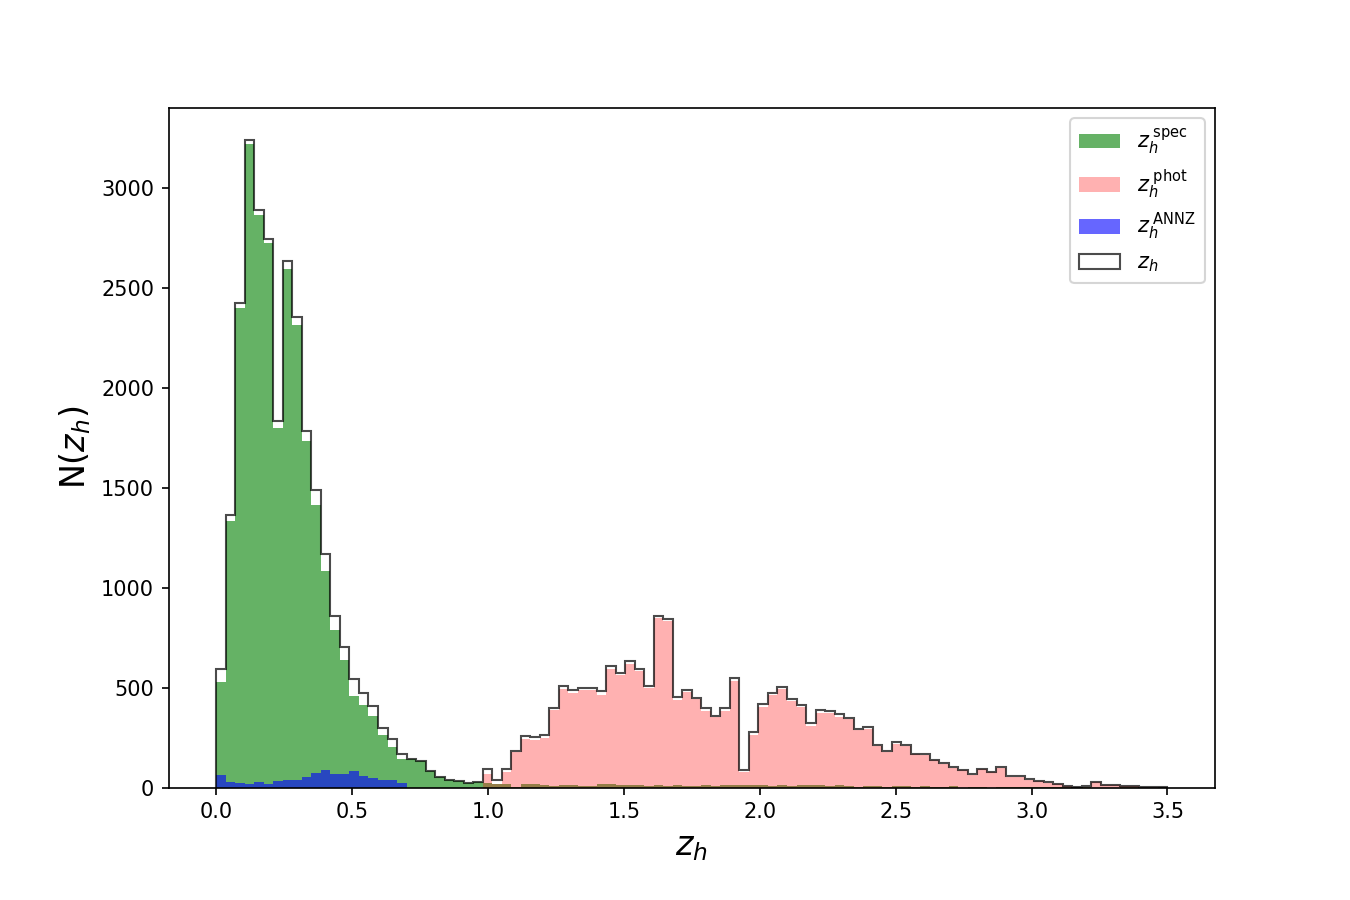
\includegraphics[width=15cm]{2_Muestras/histograma_z_hatlas_disponible.png}
    \end{center}
    \vspace*{-10mm}
    \caption{\small Histograma del \rt\ de los 47844 fuentes del proyecto \hatlas\ de los que el disponemos medidas o estimaciones  razonables del \rt\ \maths{z_{h}} de un total de 120230 para el catálogo completo. Estas fuentes se encuentran representadas en tres categorías; objetos de los que se dispone de una medida espectroscópica de confianza \maths{N({z_{h}^{\mathrm{spec}}})=28389}, objetos cuyo \rt\ tiene un nivel de confianza \maths{Q_h=1\vee2} (tratados como si hubieran sido obtenidos mediante ANNZ) \maths{N(z_{h}^{\mathrm{annz}})=931} y objetos cuyo \rt\ ha sido obtenido mediante el método descrito en la Sección~\ref{sec:3_redshift_hatlas} \maths{N(z_{h}^{\mathrm{phot}})=18524}. }
    \label{fig:histograma_z_hatlas}
\end{figure}

Por último, otro dato que es de gran importancia es el valor de la resolución angular. El valor de la FWHM\footnote{FWHM es la anchura a media altura (Full Width at Half Maximum) de la dispersión de las medidas suponiendo que se trata de una distribución normal.} para el catálogo \hatlas\ es de \maths{17.98\;\mathrm{arcsec}} en la banda de \microm{250}\footnote{El dato se encuentra en: \url{http://www.h-atlas.org/public_data/HATLAS_SDP_catalogue.README}}. Nosotros obtenemos el valor de la desviación típica como \maths{{\sigma}_{h}^{p}=\mathrm{FWHM}\times(2\sqrt{2\ln{2}})^{-1}\sim7.63\:\mathrm{arcsec}}.

\newpage

\subsection{Proyecto \gama}

\gama\ (Galaxy And Mass Assembly) es un proyecto internacional que hace uso de los más modernos observatorios espaciales y terrestres con el objetivo principal de estudiar estructuras de entre 1 kpc a 1 Mpc, lo cual incluye escalas que abarcan desde la estructura interna de las galaxias hasta cúmulos de galaxias \citep{website:Gama}. Concretamente se pretende mejorar en tres asuntos clave respecto a otros estudios:

\vspace{-3mm}

\begin{itemize}
    \setlength\itemsep{-1mm}
    
    \item Mejora de la la eficiencia espectroscópica, permitiendo el muestreo integral desde galaxias para \rt\ intermedios y mostrar esa información en un mismo estudio.
 
    \item Mejorar la resolución espacial para estudiar la estructura de las galaxias próximas y los procesos de formación galáctica.
 
    \item Mejorar el rango de la cobertura espectral.
 
\end{itemize}

Es destacable el amplio rango espectral que cubre el proyecto que abarca desde la región de Rayos X, hasta la región de radio de alta frecuencia (90 cm).  GAMA, hace uso de una amplia variedad de medidas procedentes de otros proyectos, entre los cuáles destacan:

\vspace{-3mm}

\begin{itemize}
    \setlength\itemsep{-1mm}
    
    \item Cartografiados públicos: Sloan Foundation 2.5m SDSS
    
    \item United Kingdom Infrared Telescope (UKIRT) UKIDSS-LAS
    
    \item Campañas GAMA: Galaxy Evolution Explorer (GALEX) GALEX-GAMA
    
    \item Giant Metrewave Radio Telescope (GMRT) GMRT-GAMA
    
    \item Cartografiados relacionadas con GAMA:  VLT Survey Telescope (VST) KiDS
    
    \item Visible and Infrared Survey Telescope for Astronomy (VISTA) VIKING
    
    \item The Canada France Hawaii Lensing Survey  (CFHTLenS)
    
    \item Observatorio Espacial Herschel H-ATLAS
    
    \item Australian Square Kilometre Array Pathfinder (ASKAP) DINGO
    
    \item X-ray Spectroscopy Mission and the X-ray Multi-Mirror Mission (XMM-Newton) XMM-XXL
    
    \item Wide-Field Infrared Survey Explorer (WISE)
    
\end{itemize}

El estudio espectroscópico de \gama\ cubre aproximadamente  \maths{3\times{10}^{5}} galaxias de hasta magnitud 19.8, repartidas en un área de \maths{286\;\mathrm{{deg}^{2}}}. Estas medidas son fruto de 210 noches de observación en un periodo de 7 años, desde 2008 hasta 2014, realizadas con el espectrógrafo AAOmega en el telescopio Anglo-Australiano (AAT) por miembros del equipo de GAMA. Estos datos han sido completados por datos procedentes de estudios previos como el Sloan Digital Sky Survey (SDSS), el 2dF Galaxy Redshift Survey (2dFGRS) y el Millennium Galaxy Catalogue (MGC). 

\subsubsection{Catálogo \gama\ I}

El proyecto \gama\ ha publicado dos bases de datos denominadas GAMA DR1 y GAMA DR2. La primera, fue publicada el 25 de junio de 2010 y contiene el \rt\ y otra información adicional de 114441 objetos repartidos por tres regiones, denominadas G09, G12 y G15 (Estas solapan parcialmente con las regiones que cubre el proyecto \hatlas). Estas regiones tienen una forma aproximadamente rectangular de \maths{12\times4\;\mathrm{deg}} y están situadas sobre el ecuador celeste, sumando un total de \maths{\sim144\;\mathrm{{deg}^{2}}}. El límite de magnitud para estas fuentes es de 19.4 en las regiones G09 y G15 y 19.8 en la región G12.

La segunda publicación cubre el mismo área del cielo, pero representa un conjunto de objetos más reducido de que la primera, con más información adicional. 
El límite de magnitud de los objetos pertenecientes a esta publicación es de 19.0 en la región G09 y G12 y de 19.4 para la región G15. Los datos de la región G15 son prácticamente los mismos en ambas publicaciones. 

\vspace{3mm}

\begin{figure}[htb]
    \begin{center}
         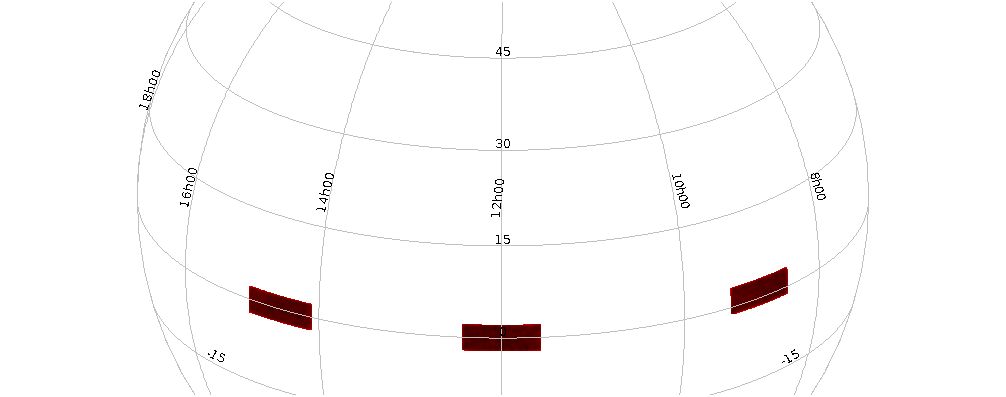
\includegraphics[width=14cm]{2_Muestras/gama.png}
    \end{center}
    
    \caption{\small Representación de los objetos publicados en el catálogo GAMA DR1 en coordenadas ecuatoriales utilizando el programa TOPCAT. De derecha a izquierda, las regiones reciben los nombres G09, G12, G15.} 
    \label{fig:TOPCAT_GAMA}
\end{figure}

En este trabajo usaremos los datos de la publicación \gama\ DR1\footnote{El fichero con los datos de esta publicación se encuentra alojado en la dirección: \url{http://www.gama-survey.org/dr1/data/GamaCoreDR1_v1.fits}}. La descripción completa de las columnas del catálogo se encuentra en el artículo \cite{article:Driver_2011}; nosotros mostramos aquí una descripción solo de las columnas que vamos a utilizar:

\begin{itemize}
    \setlength\itemsep{-1mm}
    \item GAMA\_IAU\_ID: Identificador de la fuente astronómica del catalogo GAMA asignado por la IAU.
    \item RA: Ascensión recta, en grados, de la fuente astronómica obtenida del proyecto SDSS DR6.
    \item DEC: Declinación, en grados, de la fuente astronómica obtenida del proyecto SDSS DR6.
    \item Z\_HELIO: Valores del \rt\ heliocéntrico proporcionados por el proyecto \gama. Aquellas medidas que no se encuentran disponibles se indican con un -2 o 9999.
    \item Z\_QUALITY: Etiqueta que indica la confianza que se tiene sobre los valores presentes en la columna Z\_HELIO. Nos referiremos a esta etiqueta como \maths{Q_g}.
    \item Z\_SOURCE: Etiqueta que indica la  procedencia de la medida del \rt. El criterio es el siguiente: 1 = SDSS DR6, 2 = 2dFGRS, 3 = MGC, 4 = 2SLAQ-LRG, 5 = GAMA, 6 = 6dFGS, 7 = UZC, 8 = 2QZ, 9 = 2SLAQ-QSO, 10 = NED.
    
    
\end{itemize}

El proyecto \gama\ solo proporciona medidas espectroscópicas del \rt. De las 114441 fuentes presentes en GAMA DR1, solo 59479 tienen \rt\ con factor de calidad \maths{Q_g\geq3} (los factores de calidad de los proyectos \gama\ y \hatlas\ son independientes). Los detalles relativos al factor de calidad asignado a las medidas espectroscópicas del proyecto \gama\ se encuentran en \cite{article:Driver_2011}. 

\vspace{-4mm}

\begin{figure}[htb]
    \begin{center}
         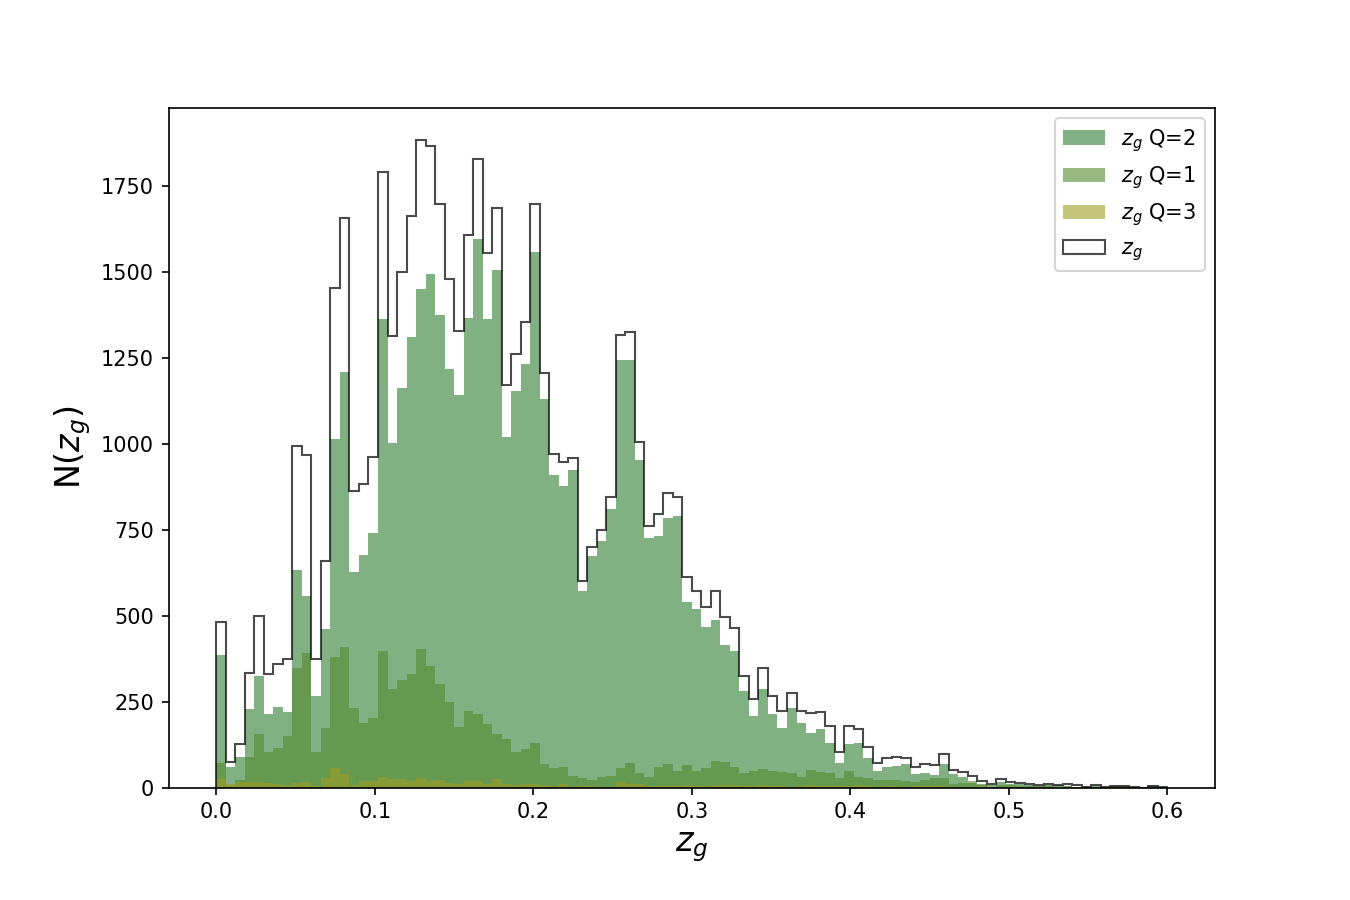
\includegraphics[width=15cm]{2_Muestras/histograma_z_gama_disponible.png}
    \end{center}
    \vspace*{-10mm}
    \caption{\small Histograma que representa el número de objetos del proyecto \gama\ de los cuales su \rt\  está disponible, \maths{N(z_{g})=59479}. Todas las medidas del \rt\ son espectroscópicas, no obstante, el proyecto les ha asignado distintos factores de calidad. Cuanto menor es el factor \maths{Q_g} mayor es la confianza que se tiene sobre esa medida. Hay 9197 con factor de calidad \maths{Q_g=1}, 49416 con \maths{Q_g=2}, y 866 con \maths{Q_g=3}. Hay objetos en ste catálogo con \maths{z_g > 0.6}, pero pero no se encuentran aquí, porque suponen una parte muy pequeña de la población representada.}
    \label{fig:histograma_z_gama}
\end{figure}

Al igual que ocurre con \hatlas, este proyecto tampoco proporciona la desviación estándar asociada a las medidas del \rt. En la Figura~\ref{fig:ajuste_error_gama} se muestra el ajuste que se ha realizado para estimar la dependencia \maths{{\sigma}^{z}} con \maths{z} a partir de una muestra de 20 objetos del catálogo \gama, con factor de calidad \maths{Q_g}=5 cuyas medidas se encuentran disponibles en NED (ver Tabla~\ref{apendice:tab:sigmas}).

\begin{figure}[htb]
    \begin{center}
         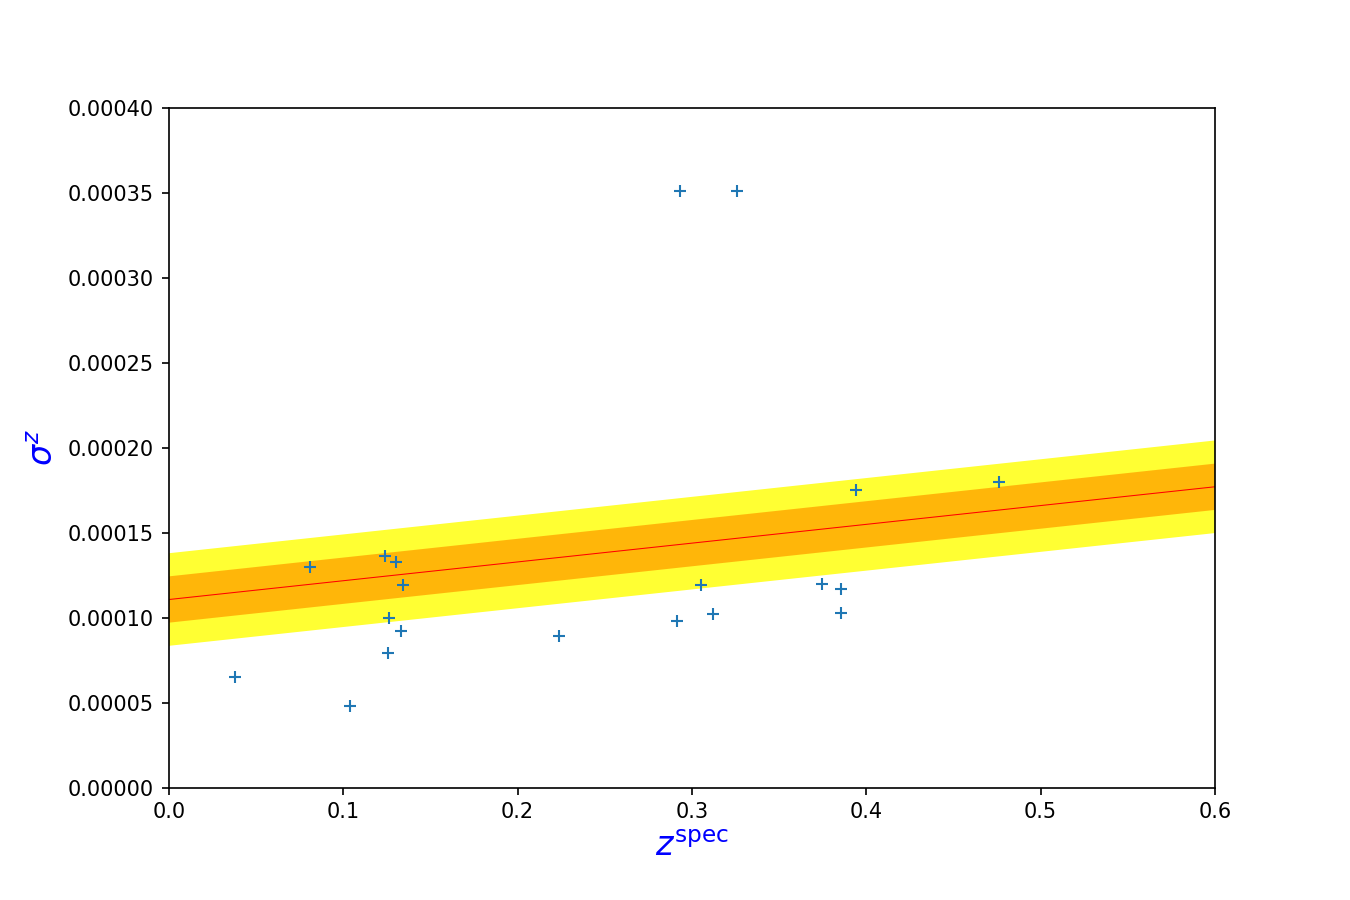
\includegraphics[width=14cm]{2_Muestras/ajuste_errores_z.png}
    \end{center}
    \vspace*{-10mm}
    \caption{\small Representación de la desviación estándar del \rt, \maths{{\sigma}^{z}} en función del \rt\ espectroscópico, \maths{{z}^{\mathrm{spec}}} de una muestra de 20 objetos del catálogo \gama\ (los 20 primeros objetos que aparecen en la Tabla~\ref{tab:ajuste_error_gama}). La recta se ha obtenido mediante un ajuste lineal de la forma \maths{{\sigma}^z= a\times(1+z)} con \maths{a} como parámetro de libre. El parámetro resultante del ajuste ha sido \maths{a=(11 \pm 1)\times{10}^{-5}}.
    \label{fig:ajuste_error_gama}}
\end{figure}

En el caso de las posiciones proporcionadas por \gama\ el valor de la \maths{\mathrm{FWHM}=0.7\;\mathrm{arcsec}}, por lo que el valor de la desviación típica en este caso es \maths{{\sigma}_{g}^{p}\sim0.30\;\mathrm{arcsec}} \citep{article:driver_2009,article:driver_2008}.

\subsection{Región de solapamiento de ambos catálogos}

Los proyectos \gama\ y \hatlas\ cubren  áreas pequeñas en comparación con la superficie total de la esfera sobre el ecuador celeste (ver Figura~\ref{fig:TOPCAT_GAMA} y Figura~\ref{fig:TOPCAT_HATLAS}). Esto permite proyectar estas regiones sobre el plano sin cambiar demasiado el valor de la superficie\footnote{La superficie de una sección esférica definida entre los paralelos 0 y
DEC y los meridianos 0 y
AR viene dada por la expresión \maths{
A_{sr}=\mathrm{AR}\times\sin{(\mathrm{DEC})}}. Si tomamos por ejemplo la región G12 que se encuentra entre los paralelos DEC=-2 y DEC=2 y meridianos RA=174 y RA=186 el área que obtenemos con la ecuación anterior es de \maths{A_{sr}\simeq0.014618666993941102\:\mathrm{sr}\simeq47.99025283641695\:\mathrm{deg^2}} mientras que al proyectar sobre una superficie plana es \maths{48\:\mathrm{deg^2}}. La diferencia entre el valor real y la aproximación es por tanto inferior a \maths{0.01\:\mathrm{deg^2}}.}.

Las áreas cubiertas por \gama\ tienen una forma que se aproxima muy bien a un rectángulo, mientras las regiones de \hatlas\ forman un polígono de 16 vértices con el que resulta más difícil trabajar. Por ese motivo, para calcular las áreas de las regiones de intersección de ambos catálogos se ha recurrido a la función \texttt{area\_region} que se encuentra definida en el Apéndice~\ref{apendice:codigo:get}. De forma resumida, lo que se hace es proyectar los puntos sobre un plano y crear una red con celdas cuadradas. Después se hace un conteo de las celdas que tienen objetos de \gama\ y de \hatlas\ a una distancia de su centro igual o inferior a la mitad de la diagonal de la celda. De esta manera se obtiene el área de las regiones de solapamiento como el producto del área de la celda por el número surgido del conteo.

Al aplicar el algoritmo para determinar el área de las regiones cubiertas por cada uno de los catálogos vemos que existen diferencias de entorno a \maths{1\:\mathrm{deg^2}} con las áreas que consideramos consideramos correctas. A partir de esta observación hemos estimado un área de intersección entre ambos catálogos de \maths{130\pm1\:\mathrm{deg^2}}.

\newpage

\begin{figure}[H]
\captionsetup[subfigure]{labelformat=empty}
%Ausencia de espacios entre los subfloat, figuras en paralelo
  \begin{center} 
  
    \subfloat[]{
     \label{subfig:region_1}
      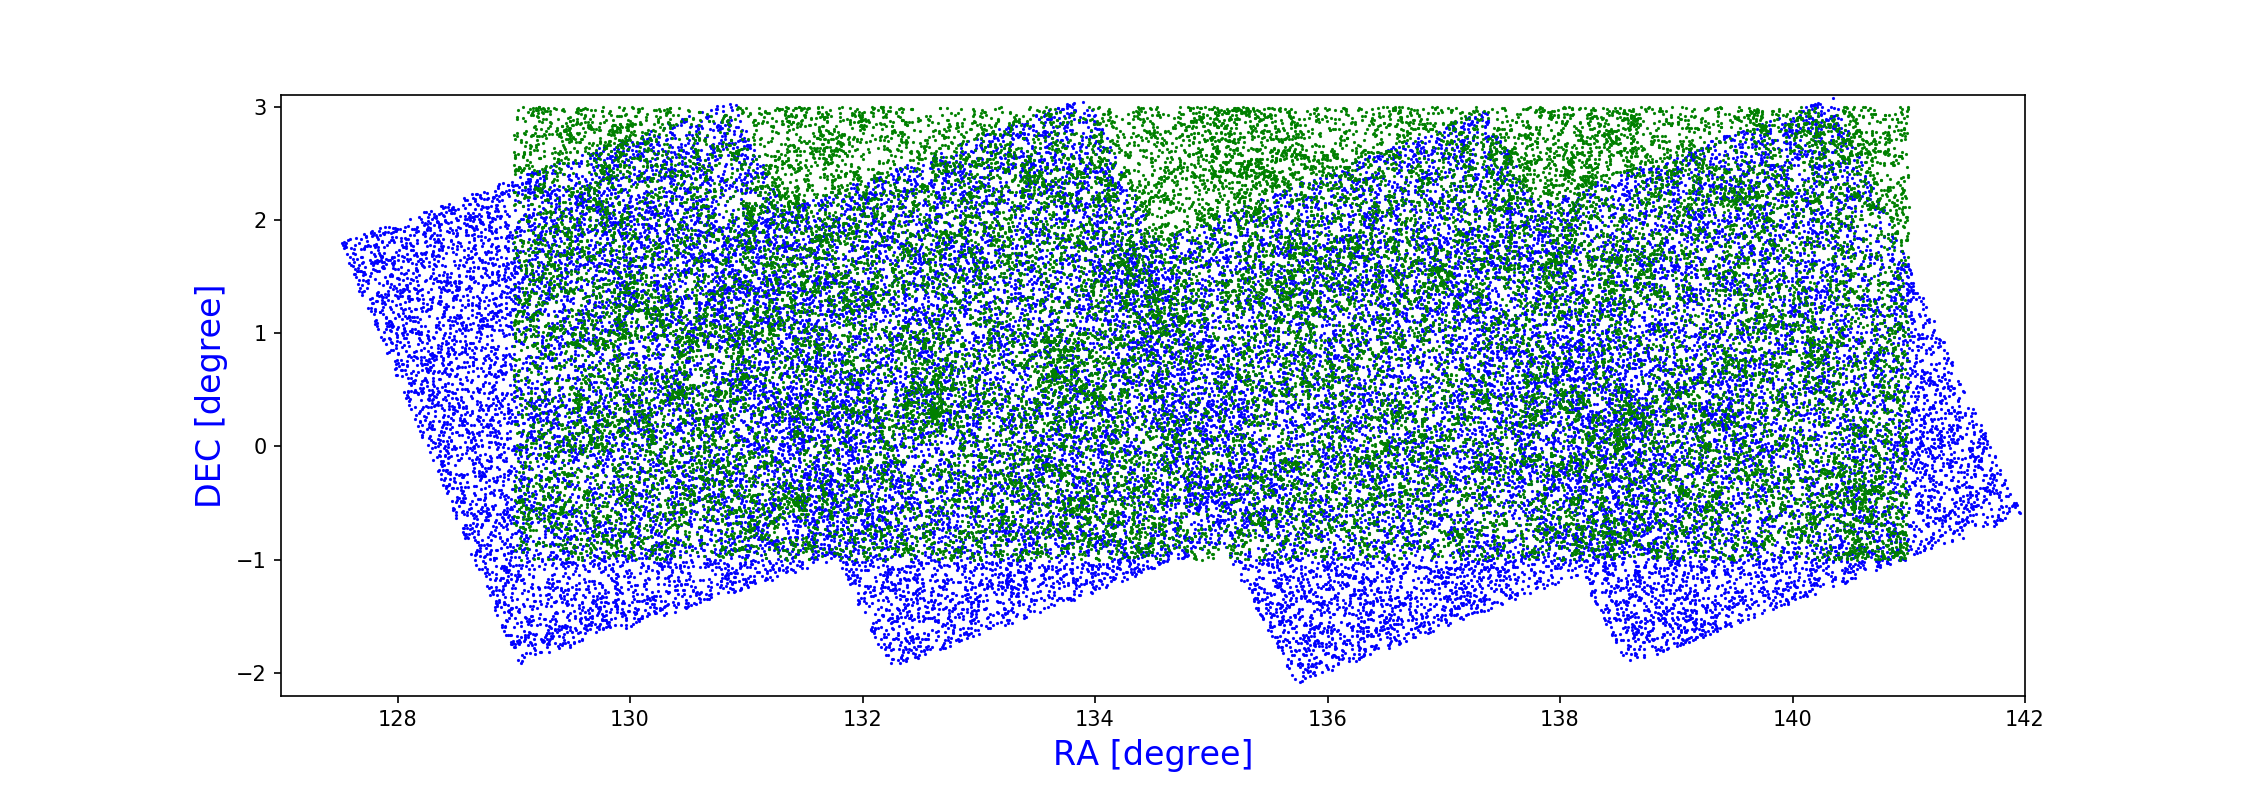
\includegraphics[width=\textwidth]{2_Muestras/region_1.png}}
      \vspace*{-10mm}
      \caption*{\small G09 (48.56 \maths{\mathrm{{deg}^{2}}}, verde) y Bloque 2 (54.15 \maths{\mathrm{{deg}^{2}}}, azul). Solapamiento: 42.96 \maths{\mathrm{{deg}^{2}}}.}
      
    \subfloat[]{
     \label{subfig:region_2}
      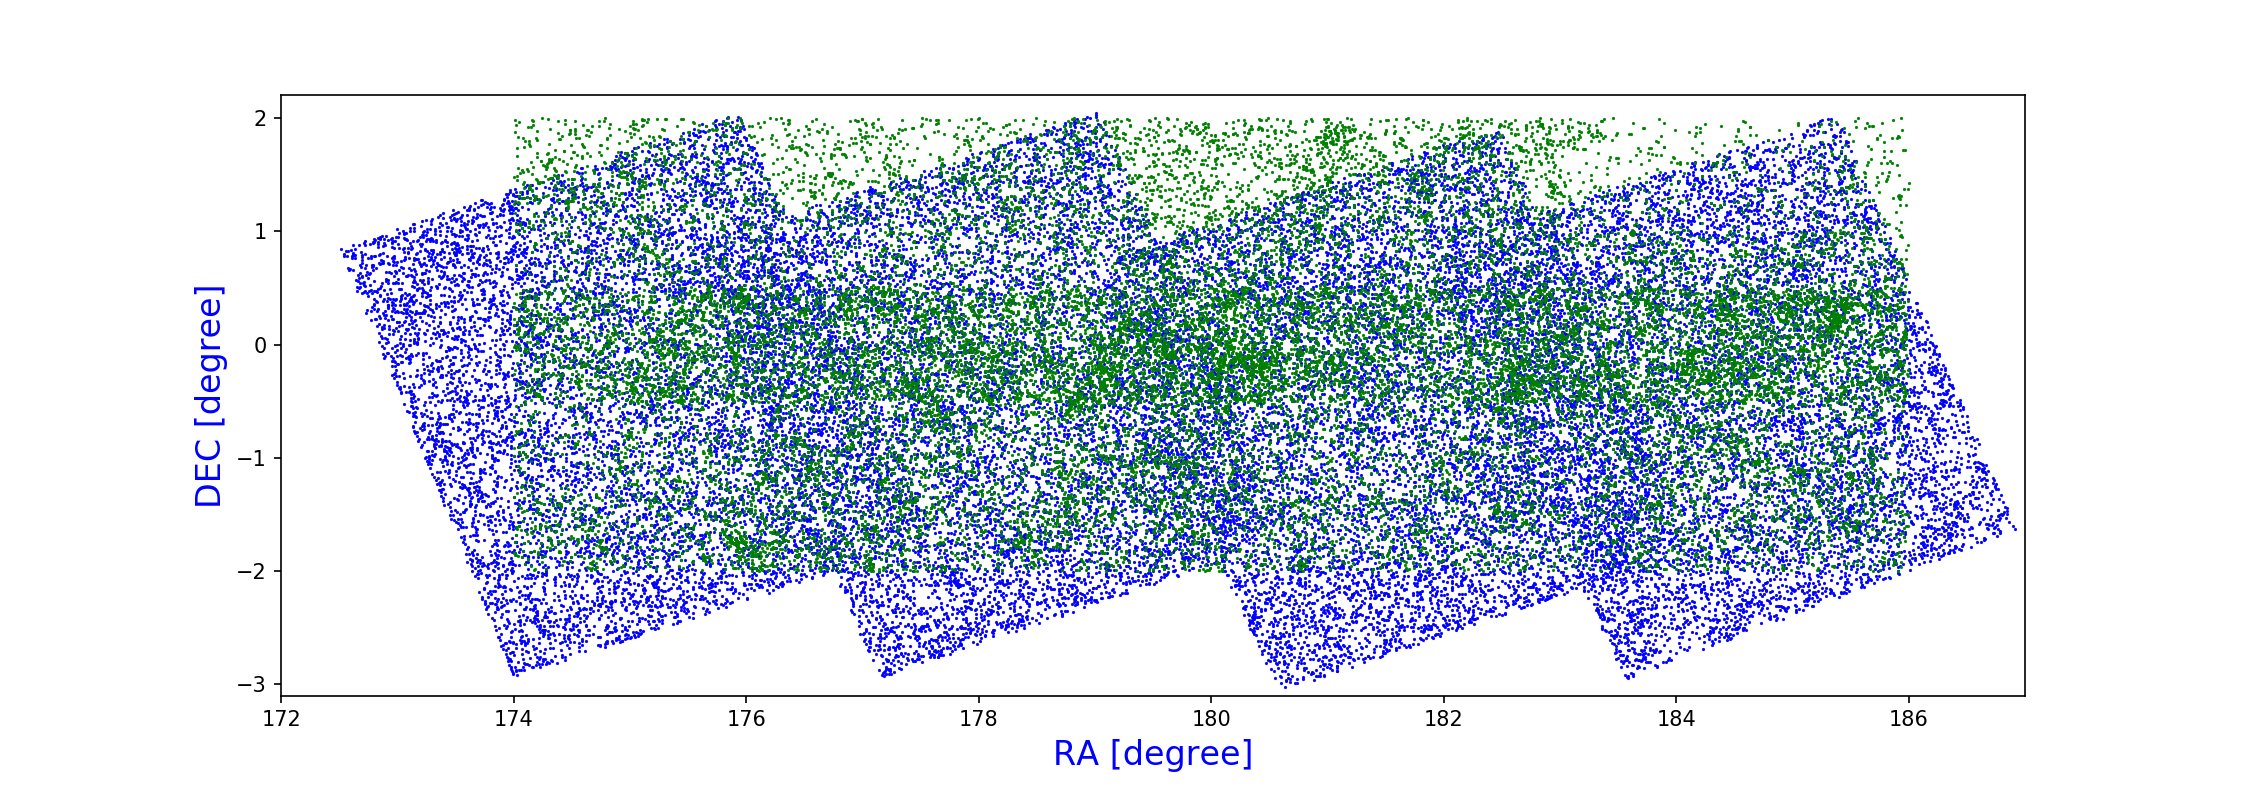
\includegraphics[width=\textwidth]{2_Muestras/region_2.png}}
      \vspace*{-10mm}
      \caption*{\small G12 (49.03 \maths{\mathrm{{deg}^{2}}}, verde) y Bloque 3  (54.40 \maths{\mathrm{{deg}^{2}}}, azul). Solapamiento: 43.46 \maths{\mathrm{{deg}^{2}}}.}
      
    \subfloat[]{
     \label{subfig:region_3}
      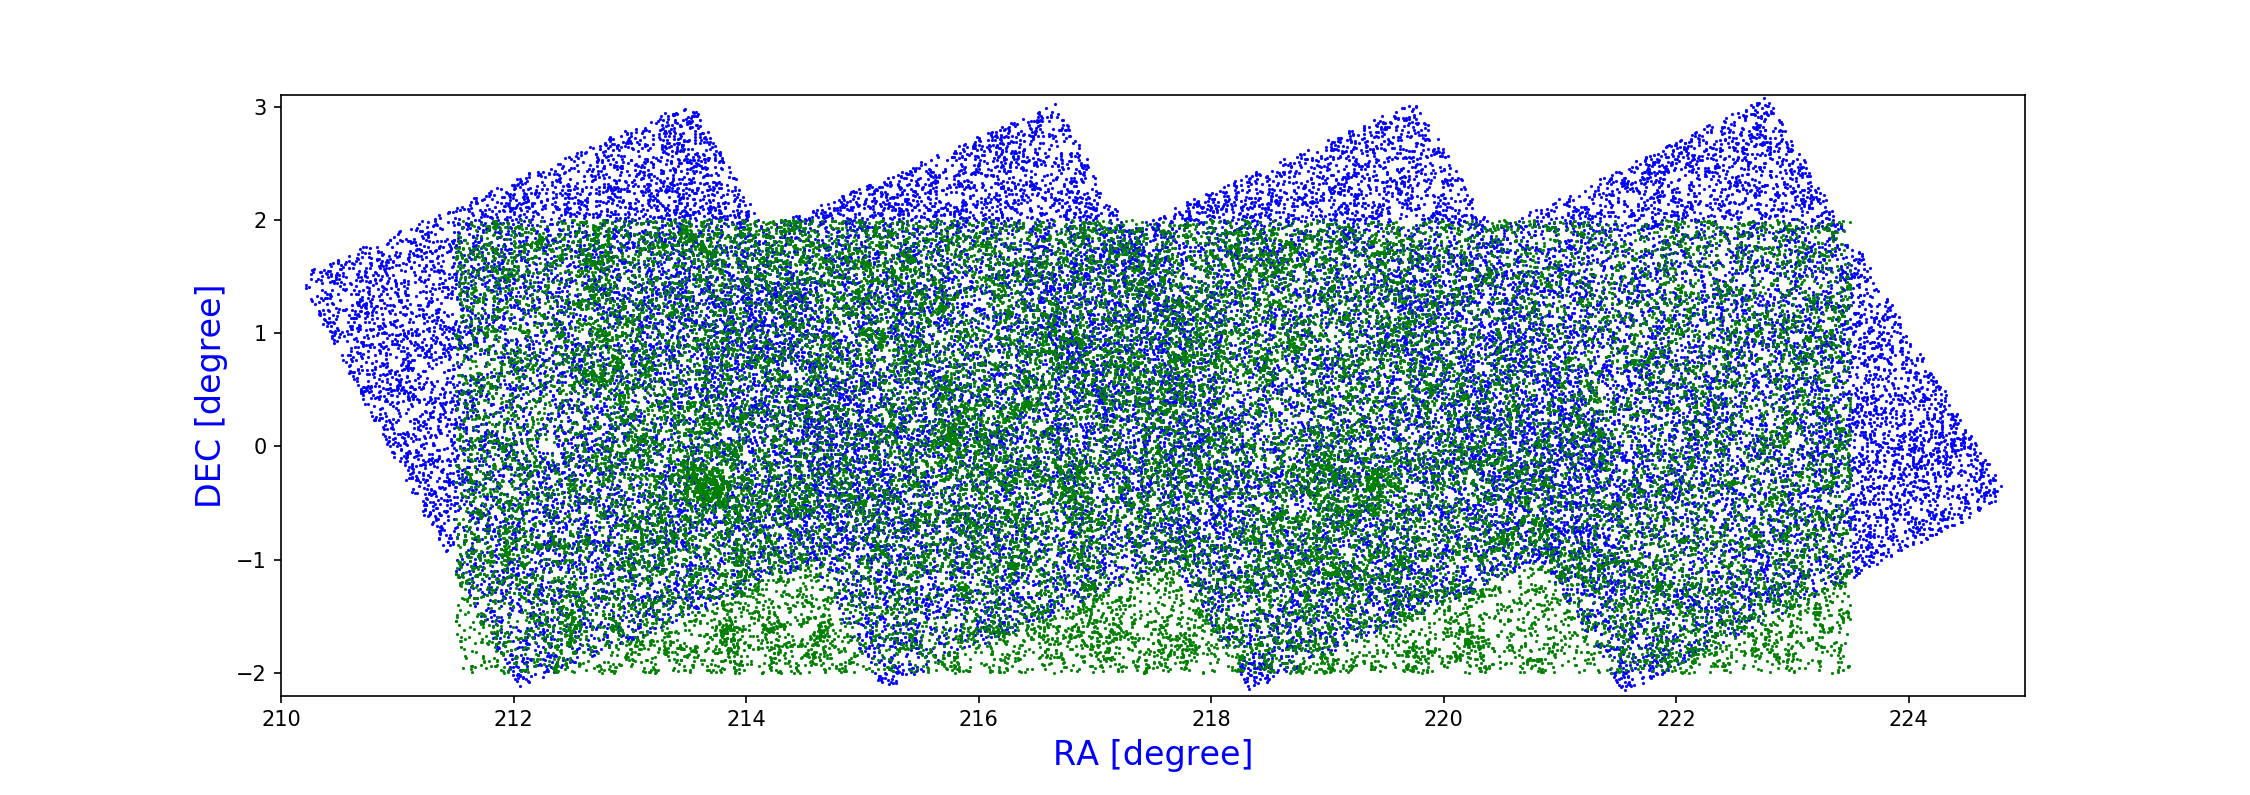
\includegraphics[width=\textwidth]{2_Muestras/region_3.png}}
      \vspace*{-10mm}
      \caption*{\small G15 (48.68 \maths{\mathrm{{deg}^{2}}}, verde) y Bloque 4 (54.80 \maths{\mathrm{{deg}^{2}}}, azul). Solapamiento: 43.88 \maths{\mathrm{{deg}^{2}}}.}
      
  \end{center}
  \caption{\small Superposición de los catálogos \gama\ (verde) y \hatlas\ (azul). Las áreas que se indican en el pie de cada imagen, se han obtenido a partir de la función \texttt{area\_region} que se encuentra definida en el Apéndice~\ref{apendice:codigo:get}. El área total cubierto por del catálogo \hatlas\ es de \maths{\sim163.35\;\mathrm{deg}^2} (según el proyecto \hatlas\ el área de los bloques 2, 3 y 4 es de \maths{161\;\mathrm{deg}^2}), el de \gama de \maths{\sim146.27\;\mathrm{deg}^2} (según \gama\ el área total de las tres regiones G09, G12 Y G15 es de \maths{144\;\mathrm{deg}^2}) y el área total de solapamiento de \maths{\sim130.3\;\mathrm{deg}^{2}}.}
  \label{fig:superposicion}
\end{figure}